\section{\unsure{I'm not quite happy with this heading yet}
	Evaluation on Different Datasets}
\label{sec:evaluation}

In a first step, the model's performance will be analyzed for different configurations of training and test data.
For training the Adam Optimizer \cite{kingma17} with an initial learning rate of $0.0002$ and $\beta_1 = 0.5$ is used for both generator and discriminator.
This particular choice of $\beta_1$ has shown to result in faster convergence.
As in the work by \citet{drover18}, the data is split up into batches of $32768$ poses for training.
Generator and discriminator are trained alternately with the same batch of poses.
Before adjusting the networks' parameters, adaptive clipping is applied to the gradients \cite[Section~3.2.1]{chorowski14}.


\subsection{Results for Training with Synthetic Data}

Later in this work, the effects of pose normalization will be analyzed.
For a meaningful comparison of normalized and non-normalized poses, in a first step the results for poses which are naturally normalized are obtained.
The normalization applied to the 2D poses consists of two parts: Centering the pose node and scaling.
As will further be elaborated in Section \ref{sec:effects-of-normalization}, the need for scaling can hardly be avoided.
Centering however can be easily avoided, when the camera projecting the 3D poses is centered at the pose's root joint.

For a fine control of the 2D poses' degree of normalization the 2D poses included in the dataset are not viable.
Hence, 2D poses are synthetically generated by projecting the monocular 3D poses available in the Human3.6M dataset.
These synthetic poses are created by "photographing" them with virtual cameras that provide the desired 2D poses.
For training and testing, cameras with integer azimuth and elevation angles randomly sampled from [0, 359] degrees and [0, 20] degrees are used.
This choice of elevation angles is based on the heuristic that in reality people are rather photographed from above than from below.
The 3D poses are first normalized such that the norm limb has length 1 and then photographed with a camera-root-joint distance of 10 units.
Thus and from the specific choice of elevation angles, in most cases the projected root limb has a length of almost 0.1 and only slight scaling is necessary.
For training, \citet{drover18} follow a similar procedure and augment synthetic 2D poses, although they use 8 fixed cameras instead of randomly sampling camera angles for each pose.

\begin{table}[]	
	\centering
	\begin{tabularx}{\textwidth}{l *{8}{Y}}
		\toprule
		Method & Direct. & Discuss & Eat & Greet & Phone & Pose & Purchase & Sit \\
		\midrule
		\citet{drover18} & 34.3 & 36.4 & 28.4 & 33.7 & 30.0 & 43.8 & 31.7 & 32.5\\
		Synthetic & 36.3 & 35.5 & 35.6 & 42.6 & 34.8 & 44.1 & 45.2 & 36.3 \\
		Human3.6M & 35.7 & 34.2 & 37.9 & 40.3 & 37.3 & 38.6 & 43.5 & 40.4 \\
		\bottomrule
		\toprule
		Method & SitDown & Smoke & TPhoto & Wait & Walk & WDog & WTog. & \textbf{Avg.}\\
		\midrule
		\citet{drover18} & 48.9 & 32.1 & 43.8 & 36.0 & 25.1 & 34.1 & 30.3 & \textbf{34.2}\\
		Synthetic & 51.9 & 41.9 & 50.8 & 43.0 & 38.5 & 49.6 & 40.8 & \textbf{41.0} \\
		Human3.6M & 59.7 & 45.0 & 52.6 & 42.2 & 32.5 & 45.8 & 36.0 & \textbf{41.2} \\
		\bottomrule
	\end{tabularx}
	\caption{
		Comparison of the MPJPEs reported by \citet{drover18} and for a rebuilt system trained with synthetic data. 
		The rebuilt system is tested with synthetic data ("Synthetic") and 2D poses from Human3.6M  \cite{ionescu14} ("Human3.6M").
		The results were obtained using \textbf{Protocol 1}. The MPJPEs are given in millimeters.
	 }
	\label{tbl:results-original-protocol1}
	\info[inline]{Augmented obtained with best.ckpt-16161 from e\_03\_07\_original.json;
		Human3.6M obtained with real 2D poses with best.ckpt-16161 from e\_03\_07\_original.json}
\end{table}
\begin{table}[]	
	\centering
	\begin{tabularx}{\textwidth}{l *{8}{Y}}
		\toprule
		Method & Direct. & Discuss & Eat & Greet & Phone & Pose & Purchase & Sit \\
		\midrule
		Synthetic & 48.8 & 51.5 & 41.5 & 57.7 & 49.4 & 54.3 & 48.8 & 50.0 \\
		Human3.6M & 86.5 & 81.7 & 65.2 & 86.6 & 82.4 & 85.2 & 93.6 & 61.3 \\
		\bottomrule
		\toprule
		Method & SitDown & Smoke & TPhoto & Wait & Walk & WDog & WTog. & \textbf{Avg.}\\
		\midrule
		Synthetic & 64.3 & 51.9 & 64.6 & 57.1 & 54.3 & 57.9 & 53.2 & \textbf{54.8} \\
		Human3.6M & 82.3 & 73.8 & 93.2 & 85.6 & 78.3 & 80.9 & 82.1 & \textbf{80.4} \\
		\bottomrule
	\end{tabularx}
	\caption{
		Comparison of the MPJPEs of the replicated system trained and tested with synthetic data and 2D poses from the Human3.6M dataset \cite{ionescu14}. 
		For \cite{drover18} only results with rigid alignment are available, which allows no fair comparison.
		The results were obtained using \textbf{Protocol 2}. The MPJPEs are given in millimeters.
	 }
	\label{tbl:results-original-protocol2}
	\info[inline]{Synthetic obtained with best.ckpt-16161 from e\_03\_07\_original.json;
	Human3.6M obtained with real 2D poses with best.ckpt-16161 from e\_03\_07\_original}
\end{table}
\begin{table}	
	\centering
	\begin{tabularx}{\textwidth}{l *{4}{Y}}
		\toprule
		Method & Acting3 & Freestyle3 & Walking2 & \textbf{Average}\\
		\midrule
		Protocol 1 & 65.5 & 74.7 & 65.7 & \textbf{68.3} \\
		Protocol 2 & 98.8 & 105.8 &  96.8 & \textbf{100.2} \\
		\bottomrule
	\end{tabularx}
	\caption{
		MPJPEs for the test data of the \textbf{TotalCapture} dataset \cite{trumble17}. The system was trained with synthetic data from Human3.6M.
		The results were obtained using the transformations of Protocol 1 and 2 as indicated. The MPJPEs are given in millimeters.
	 }
	\label{tbl:results-original-totalcapture}
	\info[inline]{Protocol 1 obtained with best.ckpt-16161 from e\_03\_07\_original.json;
	Protocol 2 obtained with best.ckpt-16161 from e\_03\_07\_original.json}
\end{table}

Table \ref{tbl:results-original-protocol1} shows the results for \textbf{Protocol 1} reported in \cite{drover18} and for the replicated system trained with synthetic data.
For the evaluation of the latter, one synthetic 2D pose is deterministically sampled from each monocular 3D pose available for Subject 11.
The results for the synthetic training data can not compete with the results presented by \citet{drover18}.
The exact source of the 6.8mm average discrepancy is not clear; the reasons can be of different origin.
\citet{drover18} don't mention whether they also use synthetic poses for testing or evaluate only on 2D poses provided in Human3.6M.
Another reason can be that before calculating the MPJPE, they apply a similarity transformation, but don't explicitly mention the Procrustes Analysis used in this work.
Further discrepancy can also arise from different internal configurations, like the exact training procedure or the applied gradient clipping.
\citet{drover18} also report a Batch Normalization Layer in each of the residual blocks, which could not be found to function during the replication of their proposed system.
Finally, extensive mining for the best performing model might also be a reason for the lower MPJPE.

The results for \textbf{Protocol 2} are given in Table \ref{tbl:results-original-protocol2}.
As \citet{drover18} also allow rigid alignment for Protocol 2 their results are not comparable to the ones obtained here.
For this protocol, rotation is not allowed to fit the estimated poses to the ground truth.
Hence the MPJPEs are approximately 14mm worse than those for Protocol 1.

Tables \ref{tbl:results-original-protocol1} and \ref{tbl:results-original-protocol2} also display evaluation results for the monocular 2D poses in the Human3.6M dataset.
For Protocol 1, the MPJPEs for the different categories are approximately as good as those for the synthetic data, for some activities even better.
In contrast to this, the results for Protocol 2 are clearly worse than those for the synthetic data.
Here, the error margin is at 25.6mm.
The key difference between Protocols 1 and 2 is that Protocol 1 allow rotation to fit the poses, as both protocols allow translation and scaling.
Hence, disregarding rotation, the results for the Human3.6M poses are overall just as good as those for the synthetic data.
Although this looks good from a theoretical perspective, for real world applications this is only helpful when the absolute rotation of the poses is not of interest.
Otherwise, only the results Protocol 2 are meaningful.

On the test data of the TotalCapture dataset, the average MPJPE for Protocol 1 is 68.3mm and for Protocol 2 100.2mm respectively (Table \ref{tbl:results-original-totalcapture}).
Apart from the aforementioned phenomenon, the key points of the joints are slightly different from the ones in Human3.6M.
Especially the angle between the hips is noticeable.
In Human3.6M, this angle is 180 degrees and the spine is perpendicular to the hips, whereas in TotalCapture the angle is substantially smaller (see Figure \ref{fig:human-totalcapture}).
Although the results are slightly worse for TotalCapture, they still show that the system generalizes to unseen data in a reasonable way.

\begin{figure}
	\centering
	\begin{minipage}{.45\textwidth}
		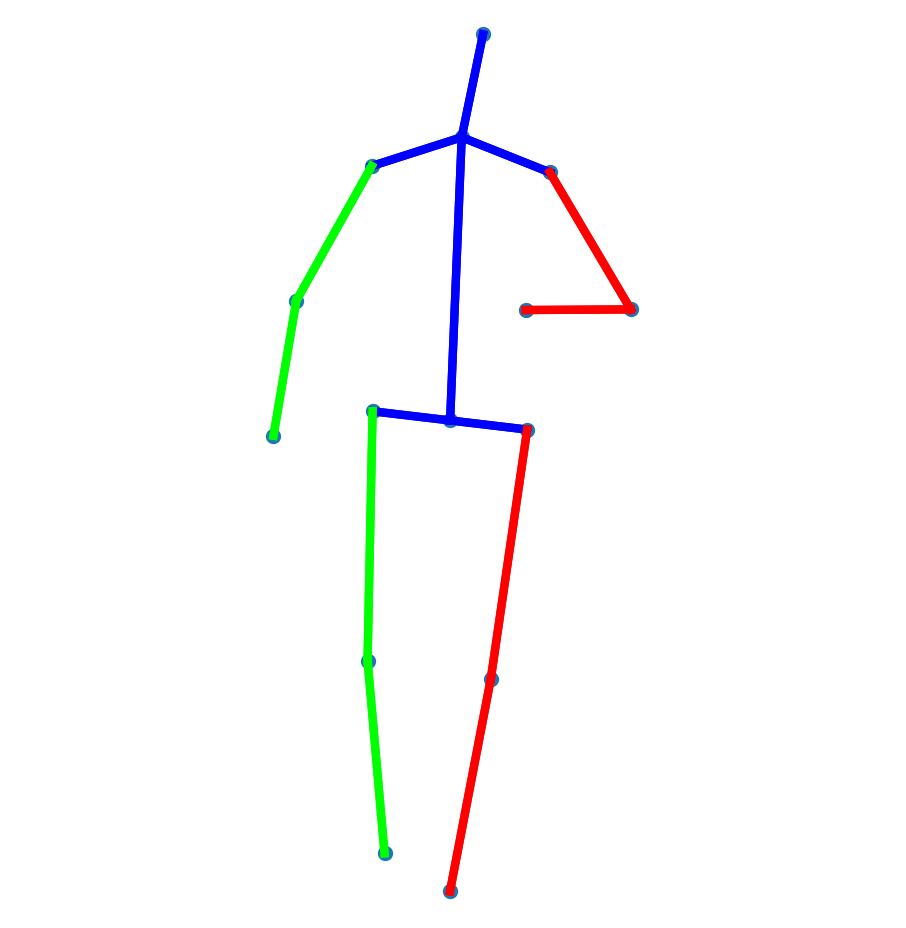
\includegraphics[width=.45\textwidth]{figures/2D_pose_human36m_1701.png}
		\scalebox{-1}[1]{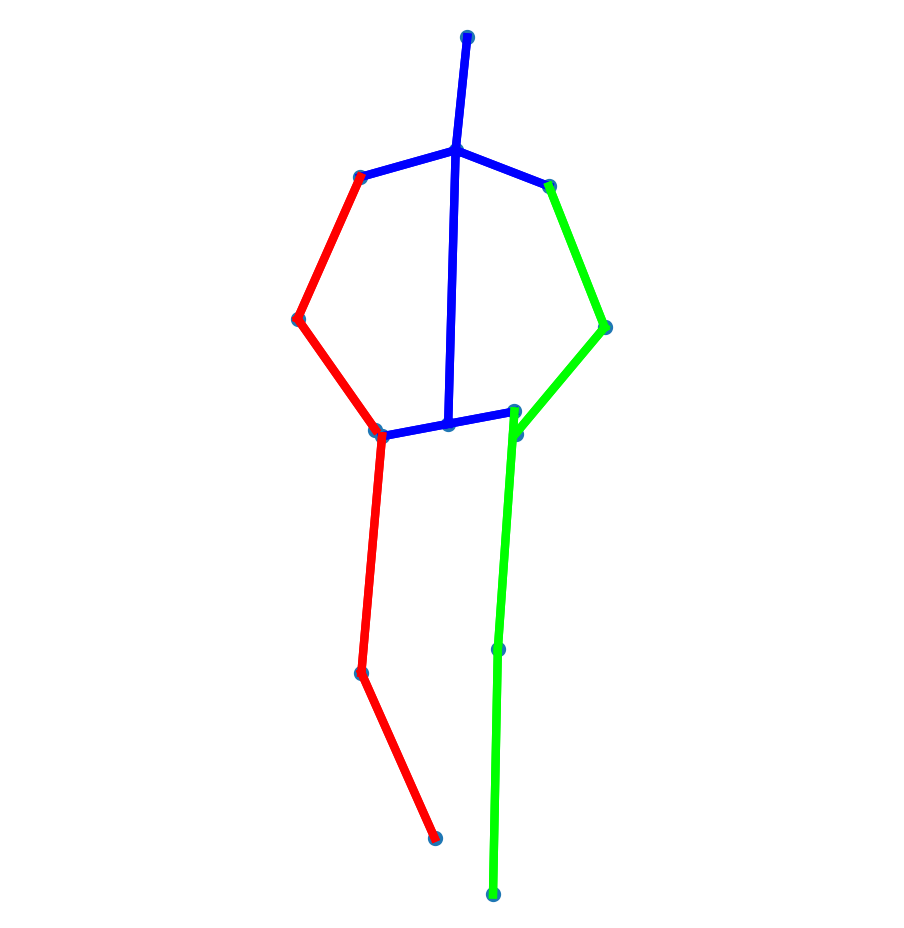
\includegraphics[width=.45\textwidth]{figures/2D_pose_human36m_4280.png}}
	\end{minipage}
	\hspace{5mm}
	\begin{minipage}{.45\textwidth}
	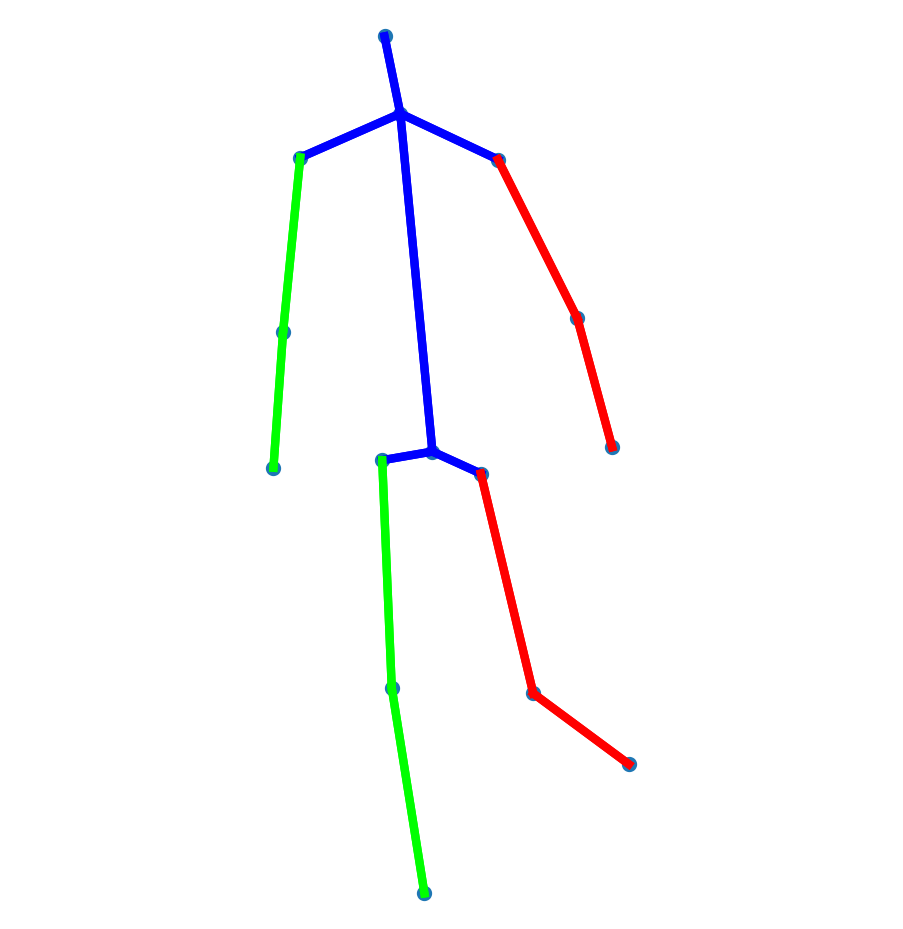
\includegraphics[width=.45\textwidth]{figures/2D_pose_totalcapture_24437.png}
	\scalebox{-1}[1]{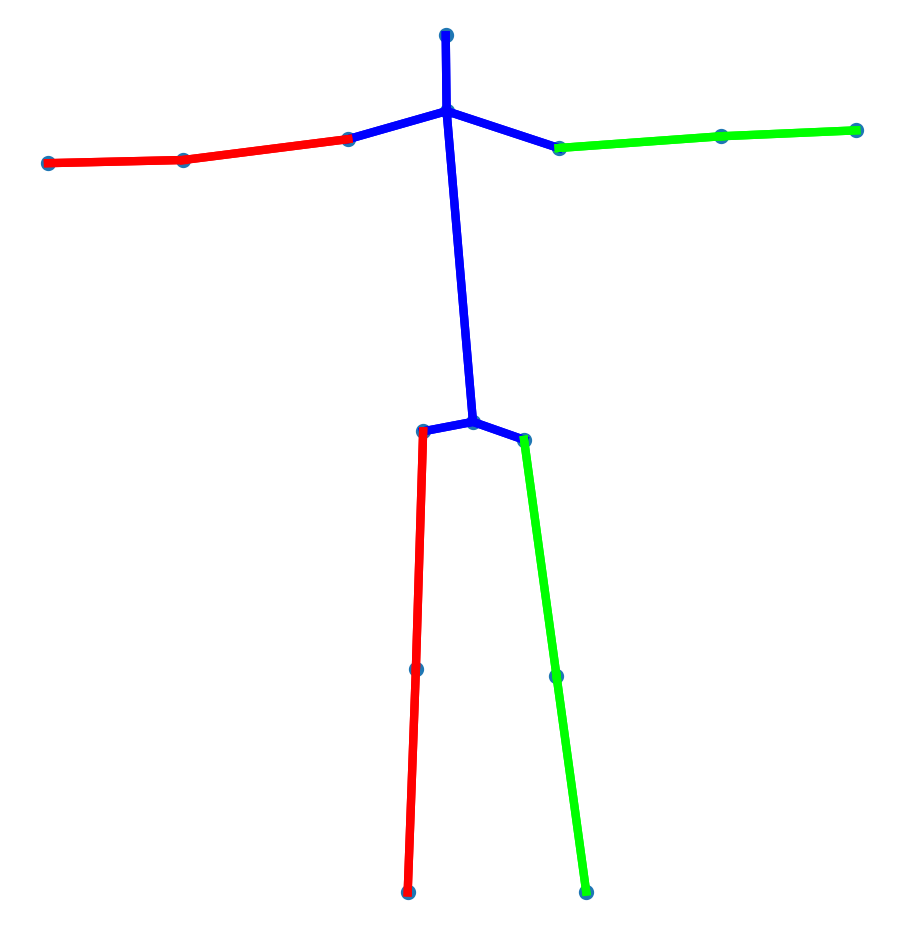
\includegraphics[width=.45\textwidth]{figures/2D_pose_totalcapture_102156.png}}
	\end{minipage}
	\caption{Comparison of two poses from the Human3.6M dataset (left) and two poses from the TotalCapture dataset (right).}
	\label{fig:human-totalcapture}
\end{figure}


\subsection{Results for Training with Augmented and Real Data}
The results for the test data of the Human3.6M dataset are not quite satisfying, as they are only useful when rotation plays no role.
The reasons for the worse results may be of different nature:
A simple explanation would be that machine learning systems usually perform better on data which is more similar to the training data.
For the synthetic testing data this is certainly the case.
On the other hand, the results for Protocol 1 show that the poses are already sensible and only seem to lack the right orientation.
Another reason might be that Human3.6M's monocular 2D poses are in fact being normalized, both in scale and position, other than the synthetic data, which is already normalized in position.

In order to figure out whether the first reason contributes to the discrepancy, the monocular 2D poses are added to the training set.
A lower MPJPE would indicate that it does.
For training, the generator receives both real and synthetic poses at a 1:1 ratio.
As described in Section \ref{sec:network}, during training the generator tries to learn the real data distribution.
In order to have a chance to achieve this, it must be able to generate poses similar to the real poses. 
This comes down to the Random Projection Layer, where the poses are projected with camera distance $d$ and a root joint offset of $0$ (which means the camera is centered at the root joint).
2D poses projected with a camera distance other than $d$ or with a non-zero root joint offset are inherently different.
This will further be elaborated on in Section \ref{sec:effects-of-normalization}.
Thus there are two options:
Projecting the generated 3D poses with a camera distance and offset similar to the real data or feeding only data to the discriminator that resembles the generator's output.
As the real camera distance might not be known in general, and offsets would still need to be sampled, the second option was chosen.
This means the discriminator still only receives synthetic poses for training.

\begin{table}[]	
	\centering
	\begin{tabularx}{\textwidth}{l *{8}{Y}}
		\toprule
		Method & Direct. & Discuss & Eat & Greet & Phone & Pose & Purchase & Sit \\
		\midrule
		Synthetic & 48.8 & 51.5 & 41.5 & 57.7 & 49.4 & 54.3 & 48.8 & 50.0 \\
		Human3.6M & 48.8 & 51.5 & 41.5 & 57.7 & 49.4 & 54.3 & 48.8 & 50.0 \\
		\bottomrule
		\toprule
		Method & SitDown & Smoke & TPhoto & Wait & Walk & WDog & WTog. & \textbf{Avg.}\\
		\midrule
		Synthetic & 64.3 & 51.9 & 64.6 & 57.1 & 54.3 & 57.9 & 53.2 & \textbf{54.8} \\
		Human3.6M & 48.8 & 51.5 & 41.5 & 57.7 & 49.4 & 54.3 & 48.8 & 50.0 \\
		\bottomrule
	\end{tabularx}
	\caption{
		Comparison of the MPJPEs of the replicated system trained with monocular 2D poses from the Human3.6M dataset and synthetic data at a 1:1 ratio.
		The results are given for synthetic data and 2D poses from the Human3.6M dataset \cite{ionescu14}.
		The results were obtained using \textbf{Protocol 2}. The MPJPEs are given in millimeters.
	 }
	\label{tbl:results-real-and-synthetic-protocol2}
	\info[inline]{}
\end{table}

Table \ref{tbl:results-real-and-synthetic-protocol2} shows the results for both synthetic data and the monocular 2D test poses from Human3.6M.
While the results for the synthetic data are approximately the same as the ones in the previous section, the results for the Human3.6M data improved by almost 8mm to 72.5mm.
This has both positive and negative consequences:
On the one hand, when the system is trained with real world data from a specific application, it will perform better in that application.
On the other hand, this shows that the system is not able to generalize to all kinds of human poses and a that part of the higher MPJPE can be attributed to a weak form of overfitting to the training data. 

\subsection{Training with augmented cameras similar to the real cameras}
Performance of system with cameras similar to the real cameras.
Results for real 2D data.

\unsure[inline]{See if it makes sense to include this section}